\section{Analyse du comportement de la chaîne de mesure}
\begin{obj}
Analyser le comportement du conditionneur associé au codeur incrémental afin de valider son implantation dans la boucle d’asservissement.
\end{obj}

Le capteur est un codeur incrémental.

\begin{marginfigure}
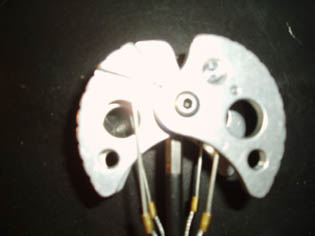
\includegraphics[width=\linewidth]{fig_03.png}
\caption{Pistes du codeur incrémental\label{fig_03}}
\end{marginfigure}

Ce codeur incrémental possède trois récepteurs :
\begin{itemize}
\item un récepteur est affecté à la piste intérieure et délivre une impulsion par tour ;
\item deux récepteurs sont placés sur la piste extérieure et sont décalés l’un par rapport à l’autre d’un quart de largeur de fente. Les signaux ainsi émis sont décalés dans le temps.
\end{itemize}

\paragraph*{Notations}

\begin{itemize}
\item $N_m$ est la fréquence de rotation en \si{tr/min} (\si{tour/min}) associée à la vitesse angulaire de l’arbre moteur $\omega_m$;
\item $a$ (respectivement $b$) est la variable binaire indiquant la réception d’un signal du premier (respectivement du deuxième) récepteur sur la piste extérieure, $a=1$ (respectivement $b=1$) si le récepteur est en face d’une fente ;
\item $\text{pulse}_a$ (respectivement $\text{pulse}_b$) est la variable binaire du front montant de $a$ (respectivement $b$), c’est-à-dire que $\text{pulse}_a=1$ (respectivement $\text{pulse}_b=1$) lorsque $a$ (respectivement $b$) passe de 0 à 1, sinon $\text{pulse}_a= 0$ (respectivement $\text{pulse}_b = 0$) ;
\item $\text{sens}_{\text{mot}}$ est la variable binaire indiquant le sens du moteur : $\text{sens}_{\text{mot}}=1$ lorsque $\omega_m>0$ et $\text{sens}_{\text{mot}}=0$ lorsque $\omega_m\leq 0$;
\item $N$ est le nombre de fentes sur la piste extérieure ($N=2500$).
\end{itemize}

Le document suivant représente l’évolution temporelle des variables $a$ et $b$ lorsque l’arbre moteur tourne à $N_m=\SI{3 000}{tr/min}$.

\begin{figure}[!h]
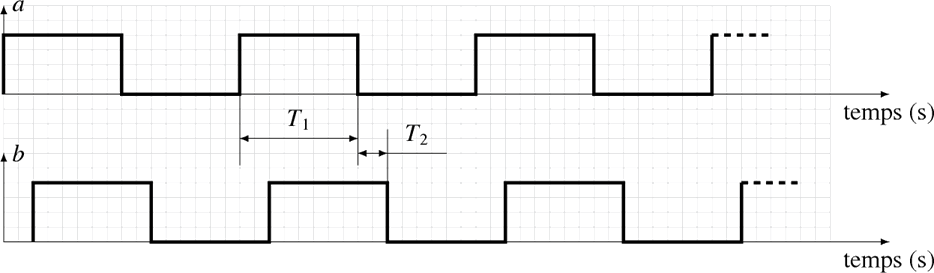
\includegraphics[width=.8\linewidth]{dr_02a.png}
\caption{Chronogramme des variables $a$ et $b$ pour $N_m = \SI{3000}{tr/min}$ \label{dr_02a}}
\end{figure}

\question{Décrire le fonctionnement du capteur et sa résolution.}

\question{Donner le chonogramme pour $\SI{1500}{tr/min}$ et $-\SI{3000}{tr/min}$.

\question{Compléter le diagramme d'état de la figure \ref{dr_03} permettant de connaître le sens du moteur.}

\begin{figure}[!h]
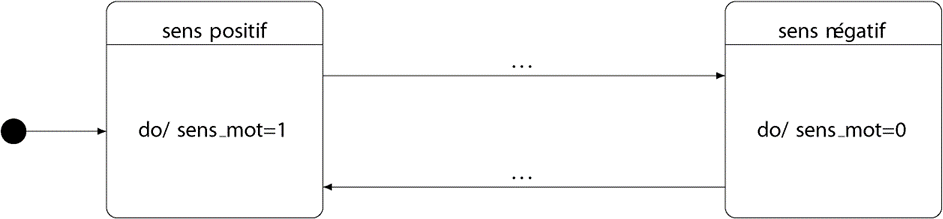
\includegraphics[width=.8\linewidth]{dr_03.png}
\caption{Diagramme d’états d’affectation de la variable $\text{sens}_{\text{mot}}$\label{dr_03}}
\end{figure}

